\documentclass[12pt,fleqn]{article}\usepackage{../common}
\begin{document}
Ders 6

Kompleks Degiskenler (Complex Variables)

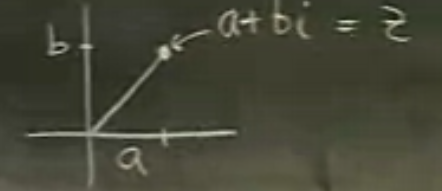
\includegraphics[height=3cm]{6_1.png}

Kompleks sayilar icinde $i$ degerini iceren sayilardir, bu deger
$\sqrt{-1}$'e esittir, bu da hayali bir sayidir. 

$z=a+bi$ sayisinin kompleks eslenigi (complex conjugate) arti
isaretini eksiye cevirerek elde edilir, $\bar{z}=a-bi$. Bu iki sayinin
carpimi, $z\bar{z} = a^2+b^2$ degeridir. Bu ozellik bir kompleks sayiyi
gercek (real) sayiya cevirmek icin kullanilan numaralardan biridir, ki
bolme isleminde bu numara kullanilir.

Mesela

\[ \frac{2+i}{1-3i} \]

Bu bolumu gerceklestirmek icin bolumun ustunu ve altini bolenin kompleks
eslenigi ile carpariz, boylece onu gercek sayi haline getiririz.

\[ \frac{2+i}{1-3i} \cdot \frac{1+3i}{1+3i}\]

Not: Sagdaki carpan faktor hem bolen hem bolunende ayni degeri tasidigi
icin aslinda 1 degerine sahip, yani bu degerle carpim yapmak aslinda sol
taraftaki faktor uzerinde ``buyukluk olarak'' hicbir degisim yaratmiyor.

\[ \frac{2+i}{1-3i} \cdot \frac{1+3i}{1+3i} = \frac{-1+7i}{10}\]


$a+bi$ formunda yazarsak

\[ \frac{-1}{10} + \frac{7}{10}i \]

Bu teknik cogunlukla lisede ogretilir. Bir diger kavram ``kutupsal form
(polar form)'' kavramidir, bu lisede ogretilebiliyor bazen, fakat ogretilen
sey bizim ihtiyaclarimizi acisindan yeterince gelismis degil. 

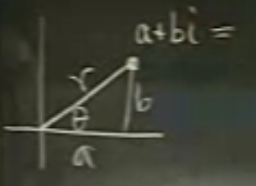
\includegraphics[height=2cm]{6_2.png}

Kutupsal form bir kompleks sayinin grafiksel gosterimi ile alakali. Eger x
ekseni $a$ ise, y ekseni $b$ ise, o zaman bir $r$ cizgisi ve $\theta$ acisi
uzerinden kutupsal forma gecilebilir. Buradan hareketle kompleks sayi su
sekilde de gosterilebilir. 

\[ a+bi = r\cos(\theta) + ir\sin(\theta) \]

\[ = r (\cos(\theta) + i\sin(\theta)) \]

Tarihten bir anektod: bu formu bulan Euler bu noktada ``parantez icindekine
$e^{i\theta}$ diyecegim'' der. Niye? Pek cok bulgu, diger matematik bu yonu
gosteriyor gibiydi. Bu matematikte onemli buluslardan biridir, ve her
acidan gormemiz, anlamamiz iyi olur. 

Bu esitlik nasil isliyor? Niye isliyor? Cunku bazi onemli ozelliklere sahip:

1. Ustel kanun (exponential law):

\[ a^x \cdot a^x = a^{x+y} \]

2. $e^{at}$, $dy/dt = ay$ diferansiyel denkleminin cozumudur. Bu ozgun
(unique) cozum degildir, ama bir baslangic sarti ekleyerek onu ozgun hale
getirebiliriz, mesela $y(0)=1$ gibi.

3. $e^x$'in turevi yine kendisidir. 

Yani

\[ e^{i\theta_1} \cdot  e^{i\theta_2} = e^{i(\theta_1 + \theta_2)}\]

\[ \frac{d}{d\theta} e^{i\theta} = i e^{i\theta} \]

Simdi bu kavramlari kullanarak Euler formunu ispatlayalim. 

Diyelim ki $\sin$, $\cos$ iceren esitligi alip ustteki carpimin icine
koyuyoruz.

\[ 
(\cos\theta_1 + i\sin\theta_1) \cdot (\cos\theta_1 + i\sin\theta_1) =
\] 

\[  
\cos\theta_1\cos\theta_2 - \sin\theta_1\sin\theta_2 +
i(\sin\theta_1\cos\theta_2 + \sin\theta_2\cos\theta_1 )
\] 

Biraz karisik gibi duruyor fakat dikkat edersek, ustteki formulun gercek
sayi kismi $\cos(\theta_1 + \theta_2)$'den ibaret (trigonometrik esitliklerden biri). 
Kompleks kismi ise $\sin(\theta_1 + \theta_2)$. O zaman elde ettigimiz \[
\cos(\theta_1+\theta_2) + i\sin(\theta_1+\theta_2) \] 
yani $e^{i(\theta_1+\theta_2)}$'in acilimi!

$e^{i\theta_1} \cdot e^{i\theta_2}$'den ise basladik, bir esitligi kullanarak, basitlestirdik, 
ve ustel kanunun soyledigi ayni sonuca erismis olduk. Demek ki $\sin$ ve $\cos$ 
iceren esitlik dogru bir esitlik.

Simdi turevi kullanarak ayni seyi ispatlamaya ugrasalim. 

\[ e^{i\theta} = \cos(\theta) + i\sin(\theta) \]

$e^{i\theta}$ nedir? Bir ustel fonksiyondur. Bu fonksiyona girdi olarak
verilen bir gercek sayidir, disari cikan ise bir kompleks sayidir. Girdi
$\theta$'dir, cikan $e^{i\theta}$'dir.

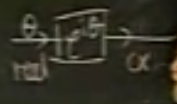
\includegraphics[height=2cm]{6_3.png}

$\theta$ yerine $t$ kullanarak aciklamaya devam edelim. Kompleks sonuc
ureten bir fonksiyonu ``kompleks degerli bir fonksiyon'' ismi verilir. $t$
girdisi alan bir kompleks degerli fonksiyon su genel formla temsil
edilebilir. 

\[ u(t) + iv(t) \]

$u$ yerine $\cos$, $v$ yerine $\sin$ oldugunu dusunebiliriz. Boyle bir
fonksiyonun turevini nasi aliriz? Her terimin teker teker turevini
alarak. Turev islemi olarak $D(..)$ kullanirsak,

\[ D(u+iv) = Du + iDv \]

O zaman su turevi alalim ($\theta$ yerine $t$ kullaniyoruz) 

\[ \frac{d}{dt}e^{it} = \frac{d}{dt}(\cos(t) + i\sin(t)) \]

\[ = -\sin(t) + i\cos(t) \]

$i$'yi disari cekelim

\[ = i \bigg( \cos(t) + i\sin(t) \bigg) \]

Bu neye esittir? $ie^{it}$ degerine! Turevi aldik, $\sin, \cos$ esitligine
atladik, ve turevi onun uzerinden hesapladik. Daha sonra
basitlestirdigimizde sonucun $e^{it}$'in bildigimiz direk turevine aynen
esit oldugunu gorduk! Bir ispat daha. 

Baslangic degerlerini dusunelim: $e^{i\cdot 0}$ neye esittir? 

Dikkat: Hemen $i \cdot 0 = 0$ ve $e$ uzeri $0$ esittir 1 cevabini
vermeyelim. Bu dogru sonuctur ama tamamiyle dogru bir mantik zinciri
degildir. Unutmayalim, $e^{i\theta}$'nin acilimi $\cos(\theta) +
i\sin(\theta)$, O zaman

\[ e^{i \cdot 0} = \cos(0) + i\sin(0) \]

$\sin(0) = 0$ olduguna gore

\[ e^{i \cdot 0} = 1 + i \cdot 0 \]

\[ = 1 +  0  = 1\]

Simdi sonuc 1 diyebiliriz.

Kutupsal forma donersek, 

\[ e^{a+ib}  = e^a \cdot e^{ib}\]

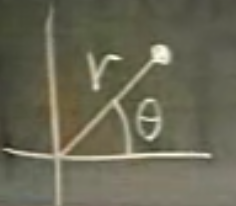
\includegraphics[height=2cm]{6_4.png}

Yani kutupsal form olarak $re^{i\theta}$. 

Bu sayinin modulusu (modulus) $r$'dir, argumani $\theta$'dir denir. Modulus
icin $|..|$ isareti, argumani icin $arg(..)$ kullanildigi da oluyor. 

Kutupsal formun avantaji nedir? Kompleks sayilarin carpilmasi sirasinda cok
ise yarar. Bu formda calisiyorsak islemler cok kolaylasiyor ve sonuc cok
temiz bir sekilde geliyor. Mesela

\[ r_1 e^{i\theta_1} \cdot r_2 e^{i\theta_2} = r_1r_2 e^{i(\theta_1+\theta_2)}\]

Gordugumuz gibi hemen moduluslari carpiyoruz, argumanlari (acilari)
topluyoruz. Buna bakarak sonucun geometrik icerigi son derece acik. Eger 

\[ (a+bi)(c+di) \]

islemini yapsaydik, karmakarisik sonuclar elde edecektik.

Bazi Ekler 

Bir kompleks sayi $a+ib$'yi aslinda bir vektor gibi gormek faydali
olabilir. Vektor dunyasinda mesela $a\vec{i} + b\vec{j}$ ifadesi vardir
(dikkat bu $\vec{i}$ kompleks i degil), ve bu ifade de bir toplam olarak
gosterilir. Dusunsel bir benzerlik var, bir eksende $a$ adimi atiyoruz,
digerinde $b$ adimi atiyoruz, ve gittigimiz yer vektorel toplamin
gosterdigi yer.

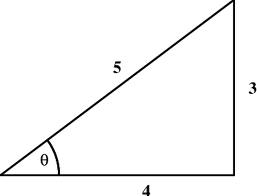
\includegraphics[height=2cm]{345.png}

Buradan hareketle toplam vektorun isaret ettigi noktayi acisal olarak ta
gosterebiliriz, ki kutupsal form buradan ileri geliyor. Eger $3 + 4i$ varsa
mesela (ustteki ucgene dikkat), $r$'nin 5 oldugunu hesaplayabiliriz, ve
oradan kenarlari bu tek uzunluga referans ederek acisal olarak ta
gosterebiliriz:

\[ z = 5(\cos\theta + i \sin\theta ) \]

Simdi diger bir yonden, Euler Esitligi devreye girebilir. Bu esitlik
parantez icinin $e$'nin ustu olarak gosterilebilecegini soylemistir!
Boylece ifade daha basitlesiyor.

\[ z = 5e^{i\theta} \]

Bu noktada bir dikkat edilecek nokta daha:

Derste bir kompleks sayinin {\em ustel olarak kullanilabilecegi}
belirtildi, mesela $e^{a+ib}$ gibi, bu baska bir sey. 


Ustel Form ve Calculus

Ustel formu kullanarak Calculus'taki bazi esitlikleri hatirlamanin,
turetmenin ne kadar kolay olduguna bakalim simdi. Mesela

\[ \int e^{-x}\cos(x) dx \]

Bunu tabii ki parcali entegral kullanarak cozebilirdik. Fakat parcali
entegrali iki kere kullanmamiz gerekirdi, biraz giriftli bir islem
olurdu. Onun yerine kompleks sayilari hemen kullanalim. 

Formule bakalim ve formuldeki $\cos(x)$'i bir kompleks sayi olan $e^{ix}$'in
$\cos(..)$ bolumu olarak gorelim. O zaman $e^{-x}\cos(x)$ carpimini
$e^{-x}Re(e^{ix}) $ olarak gorebiliriz. $Re$ tabiri bir kompleks sayinin
``reel bolumu'' anlamina geliyor. Hatta $e^{-x}$ zaten reel bir sayi
olduguna gore $Re(e^{-x}e^{ix})$ sozunu de soyleyebiliriz. Entegral icin
iste bu mantigi yurutuyoruz.

\[ e^{-x}e^{ix} = e^{-x + ix} = Re(e^{(-1+i)x}) \]

\[ \int e^{-x}\cos(x) dx = Re (\int e^{(-1+i)x} dx) \]

Bu isleme ``entegrali komplekslesirmek'' adi veriliyor, onumuzde olan
tamamen reel sayili bir formulu cozmek yerine, onu sanki kompleks bir
sayinin reel kismiymis gibi gorerek cozuyoruz. Bunu niye yapiyoruz? Cunku
ustel (exponential) bir sayiyi entegre etmek cok kolay!

\[ \int e^{(-1+i)x} dx = \frac{e^{(-1+i)x}}{-1+i}\]

Bu formulun reel kismini istiyoruz, onu nasil elde ederiz? Iste kompleks
sayilari bolebilme yetenegi simdi faydali olacak.

\[  \frac{e^{(-1+i)x}}{-1+i} = \frac{1}{-1+i} e^{-x}(\cos(x) + i\sin(x))\]

Bolenin eslenigi (conjugate) $-1-i$, onunla bolen ve boluneni
carpiyoruz.

\[ (-1+i)(-1-i) = 1-i^2-i+i = 1-(-1) = 1+1 = 2\]

Demek ki ustteki formul

\[ = \frac{-1-i}{2} e^{-x}(\cos(x) + i\sin(x)) \]

Bu formulun reel bolumu? $e^{-x}$ ve $1/2$ zaten reel carpimlar oldugu icin
onlari kenara alalim simdilik. Sadece su kismin reel bolumunu bulmaliyiz.

\[ = (-1-i)(\cos(x) + i\sin(x)) \]

Carpimi yaparken $i$ iceren terimleri atlarsak, geriye kalanlar

\[ -\cos(x) + \sin(x) \]

Kenara aldigimiz reel ifadeleri geriye getirirsek, entegralin sonucu

\[ \frac{e^{-x}}{2}(-\cos(x) + \sin(x)) \]

olacaktir. 

Kompleks sistemine bu sekilde gelip gitmek ODE dunyasinda onemli bir
yetenek. Mesela $e^{x}$ ve $\cos$ yanyana gorunce, hocanin aklina hemen
kompleks sisteme gitmek geliyor. 

Kompleks Kokleri Bulmak

Temel problem 1'in n'inci koklerini bulmaktir, yani $\sqrt[n]{1}$. Reel
dunyada sonuc kac tanedir? Bazen bir tane, 1'in kendisi, bazen 2 tane:
sonucun kac tane oldugu $n$'in cift mi tek mi sayi olduguna gore degisir.

Kompleks dunyada sonuc $n$ tanedir. Bu cevaplar nerededir? Geometrik olarak
bunu gormek kolay. Birim cemberi cizip mesela 5 parcaya bolelim:

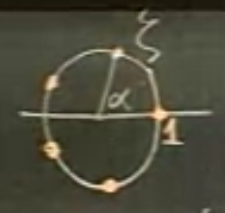
\includegraphics[height=3cm]{6_5.png}

$\alpha$ acisi nedir? Radyan olarak 

\[ \alpha = \frac{2\pi}{5} \]

Geometrik olarak bariz bir sekilde bu noktalar aradigimiz 5 tane 5'inci
kok. Diyelim ki koklerden birincisi $\zeta$ noktasinin 5 ustu nedir?
Modulus yani $r$ degeri 1, cember birim cember, bu normal, $\zeta$'yi yazalim:

\[ \zeta = e^{i\frac{2\pi}{5}} \]

O zaman

\[ 
\zeta^5 = (e^{i\frac{2\pi}{5}})^5 = e^{i\frac{2\pi}{5} \cdot 5} = e^{i2\pi} =
1 
\]

Bu cember uzerinde $2\pi$ 0'a tekabul ediyor, bir tur atip geri donduk. 

Problemler 2, 6d

Bu problemde bir kompleks ustel sayinin grafiklenmesi isleniyor. Gormek
icin MIT OCW ODE Mathlet sayfasindan erisilebilecek ``Complex Exponential''
programina gidilmesi soyleniyor. Bu program bir Applet, biz programi Python
ile tekrar kodladik. Programin alt kisminde gorulen iki ayar ile degisik a
ve b degerleri denenebiliyor. Sagdaki $e^{(a+bi)t}$'nin hesaplanabilmesi
icin su acilimi kullandik:

\[ e^{(a+bi)t} = e^{at} e^{bit}\]

\[ = e^{at} (\cos(bt) + i\sin(bt) \]

\[ = e^{at}\cos(bt) + e^{at} i\sin(bt) \]

Reel kismi (x ekseni) hesaplarken $e^{at}\cos(bt)$, hayali kismi (y ekseni)
hesaplarken $e^{at} i\sin(bt)$ formulundeki $i$ haricinde geri kalan terimleri
hesapliyoruz.

\begin{minted}[fontsize=\footnotesize]{python}
#
# MIT OCW ODE Mathlet Complex Exponentials replacement in 
# Python
#
from pylab import *
from matplotlib.widgets import Slider

ax = subplot(121)
subplots_adjust(left=0.1, bottom=0.25)
l1, = plot(None,None, lw=2, color='red')
axis([-1, 1, -8, 8])
title ('$(a + bi)t$', color='blue')
grid()

ax = subplot(122)
subplots_adjust(left=0.1, bottom=0.25)
l2, = plot(None,None, lw=2, color='red')
axis([-3, 3, -3, 3])
title ('$e^{(a + bi)t}$', color='blue')
grid()

axcolor = 'lightgoldenrodyellow'
axa = axes([0.15, 0.1, 0.65, 0.03], axisbg=axcolor)
axb  = axes([0.15, 0.15, 0.65, 0.03], axisbg=axcolor)

slidera = Slider(axa, 'a', -1.0, 1.0, valinit=0)
sliderb = Slider(axb, 'b', -8.0, 8.0, valinit=0)

def update(val):
    a = slidera.val
    b = sliderb.val
    t = arange(-1.0, 1.0, 0.001)
    l1.set_xdata(t)
    l1.set_ydata((b/a)*t)

    t = arange(-3.0, 3.0, 0.001)
    l2.set_xdata(exp(a*t)*cos(b*t))
    l2.set_ydata(exp(a*t)*sin(b*t))
    draw()
    
slidera.on_changed(update)
sliderb.on_changed(update)

plt.savefig('compexp.png')
\end{minted}

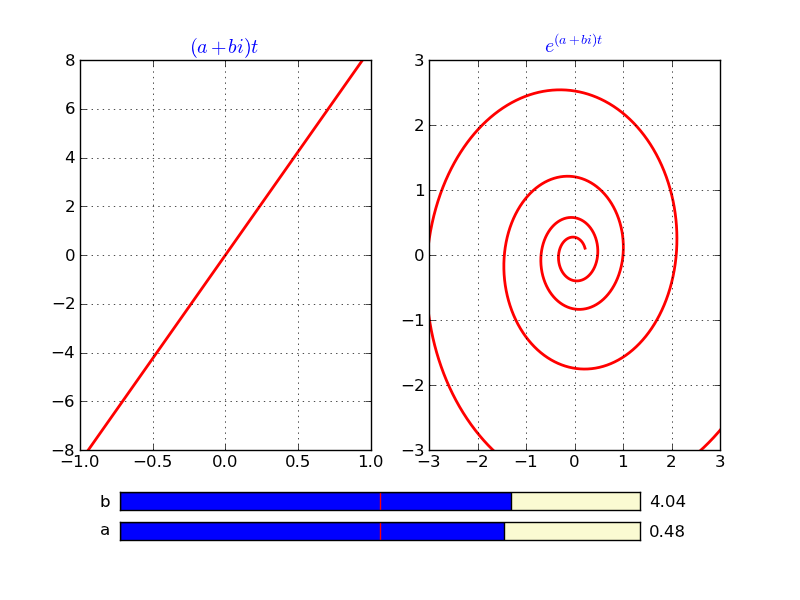
\includegraphics[height=7cm]{compexp.png}

Problemler 2, 7b

$\dot{z} + 3z = e^{2it}$ denkleminin $we^{2it}$ formunda cozumunu bul, ki
bu formda $w$ bir kompleks sayidir. Genel cozum nedir? 

Bu problem ders notlarinda daha once verilen $y' + ky = q_e(t)$ formuna
benzer. Entegre edici faktor kullanarak cozebiliriz. 

Entegre edici faktor: $e^{\int 3 dt}$ = $e^{3t}$. Iki tarafi da bu faktor
ile carpalim. 

\[ \dot{z}e^{3t} + 3e^{3t}z = e^{2it}e^{3t} \]

\[ (ze^{3t})' = e^{(3+2i)t} \]

Iki tarafin entegralini alirsak

\[ \int (ze^{3t})' = \int e^{(3+2i)t} \]

\[ ze^{3t} =  \frac {e^{(3+2i)t}}{(3+2i)} + c\]

Bolende olan kompleksligi yukari cikarmak icin kompleks eslenigi ile
carpma numarasini kullanalim. 

\[ =  \frac {e^{(3+2i)t}(3-2i)}{(3+2i)(3-2i)} + c\]

\[ =  \frac {e^{(3+2i)t}(3-2i)}{13} + c\]

\[ z =  \frac {e^{(3+2i)t}e^{3t}(3-2i)}{13} + c e^{-3t}\]

\[ z = \frac {(3-2i)}{13} e^{2it} + c e^{-3t}\]



\end{document}

